\documentclass[practic, labs]{BMSTU-IU7}

\usepackage{biblatex}
\usepackage{listings}
\usepackage{csvsimple}
\usepackage{caption}
\usepackage{pgfplots}
\usepackage{graphicx}
\pgfplotsset{compat=1.9}

\usepackage{geometry}
\geometry{verbose,a4paper,bmargin=2cm}

\newcommand{\code}[1]{\texttt{#1}}

\lstset{
	language=C++,
	numbers=left,
	captionpos=t,
	frame=single,  % Отображение рамки вокруг кода
	backgroundcolor=\color{white}
}

\student{Дьяченко А. А.}
\group{ИУ7-53Б}
\labsNumber{4}
\theme{<<Параллельные вычисления на основе нативных потоков>>}
\speciality{<<Анализ алгоритмов>>}
\supervisor{Строганов Д. В.}

\addbibresource{biblio.bib}


\begin{document}
	\maketitle

	\setcounter{page}{3}
\renewcommand{\contentsname}{Содержание}
\tableofcontents
	\section*{ВВЕДЕНИЕ}
\addcontentsline{toc}{section}{ВВЕДЕНИЕ}

<<<<<<< HEAD:passed/lab_01/report/src/02-intro.tex
Целью данной лабораторной работы является изучение расстояния Левенштейна и Дамерау~---~Левенштейна.

Расстояние Левенштейна (редакционное расстояние) и его модификация - расстояние Дамерау~---~Левенштейна, представляют собой метрики, используемые для измерения различий между двумя последовательностями символов.
=======
Целью данной лабораторной работы является изучение расстояния Левенштейна и Дамерау--Левенштейна.

Расстояние Левенштейна (редакционное расстояние) и его модификация - расстояние Дамерау--Левенштейна, представляют собой метрики, используемые для измерения различий между двумя последовательностями символов.
>>>>>>> 786b864 (lab_01 almost passed):lab_01/report/src/02-intro.tex
Они определяют минимальное количество односимвольных операций (вставка, удаление, замена и транспозиция), необходимых для преобразования одной последовательности символов в другую.
Эти метрики были разработаны советским математиком Владимиром Левенштейном в 1965 году и модифицированы впоследствии с учетом операции транспозиции символов, получив название расстояния Дамерау--Левенштейна.

Расстояние Левенштейна и его модификация имеют широкий спектр применений в различных областях, включая компьютерную лингвистику (автозамена, исправление ошибок), биоинформатику (анализ генома, белковых последовательностей).

Задачи лабораторной работы:
\begin{itemize}
    \item реализация алгоритмов с использованием динамического программирования;
    \item сравнение требуемого времени выполнения в тактах процессора и занимаемой памяти;
    \item подготовка отчёта по лабораторной работе.
\end{itemize}


	\section*{Выполнение задания}
\addcontentsline{toc}{section}{Выполнение задания}

На рисунке \ref{fig:photo} представлена реализация алгоритма поиска подстроки в строке методом полного перебора.

\begin{figure}
	\centering
	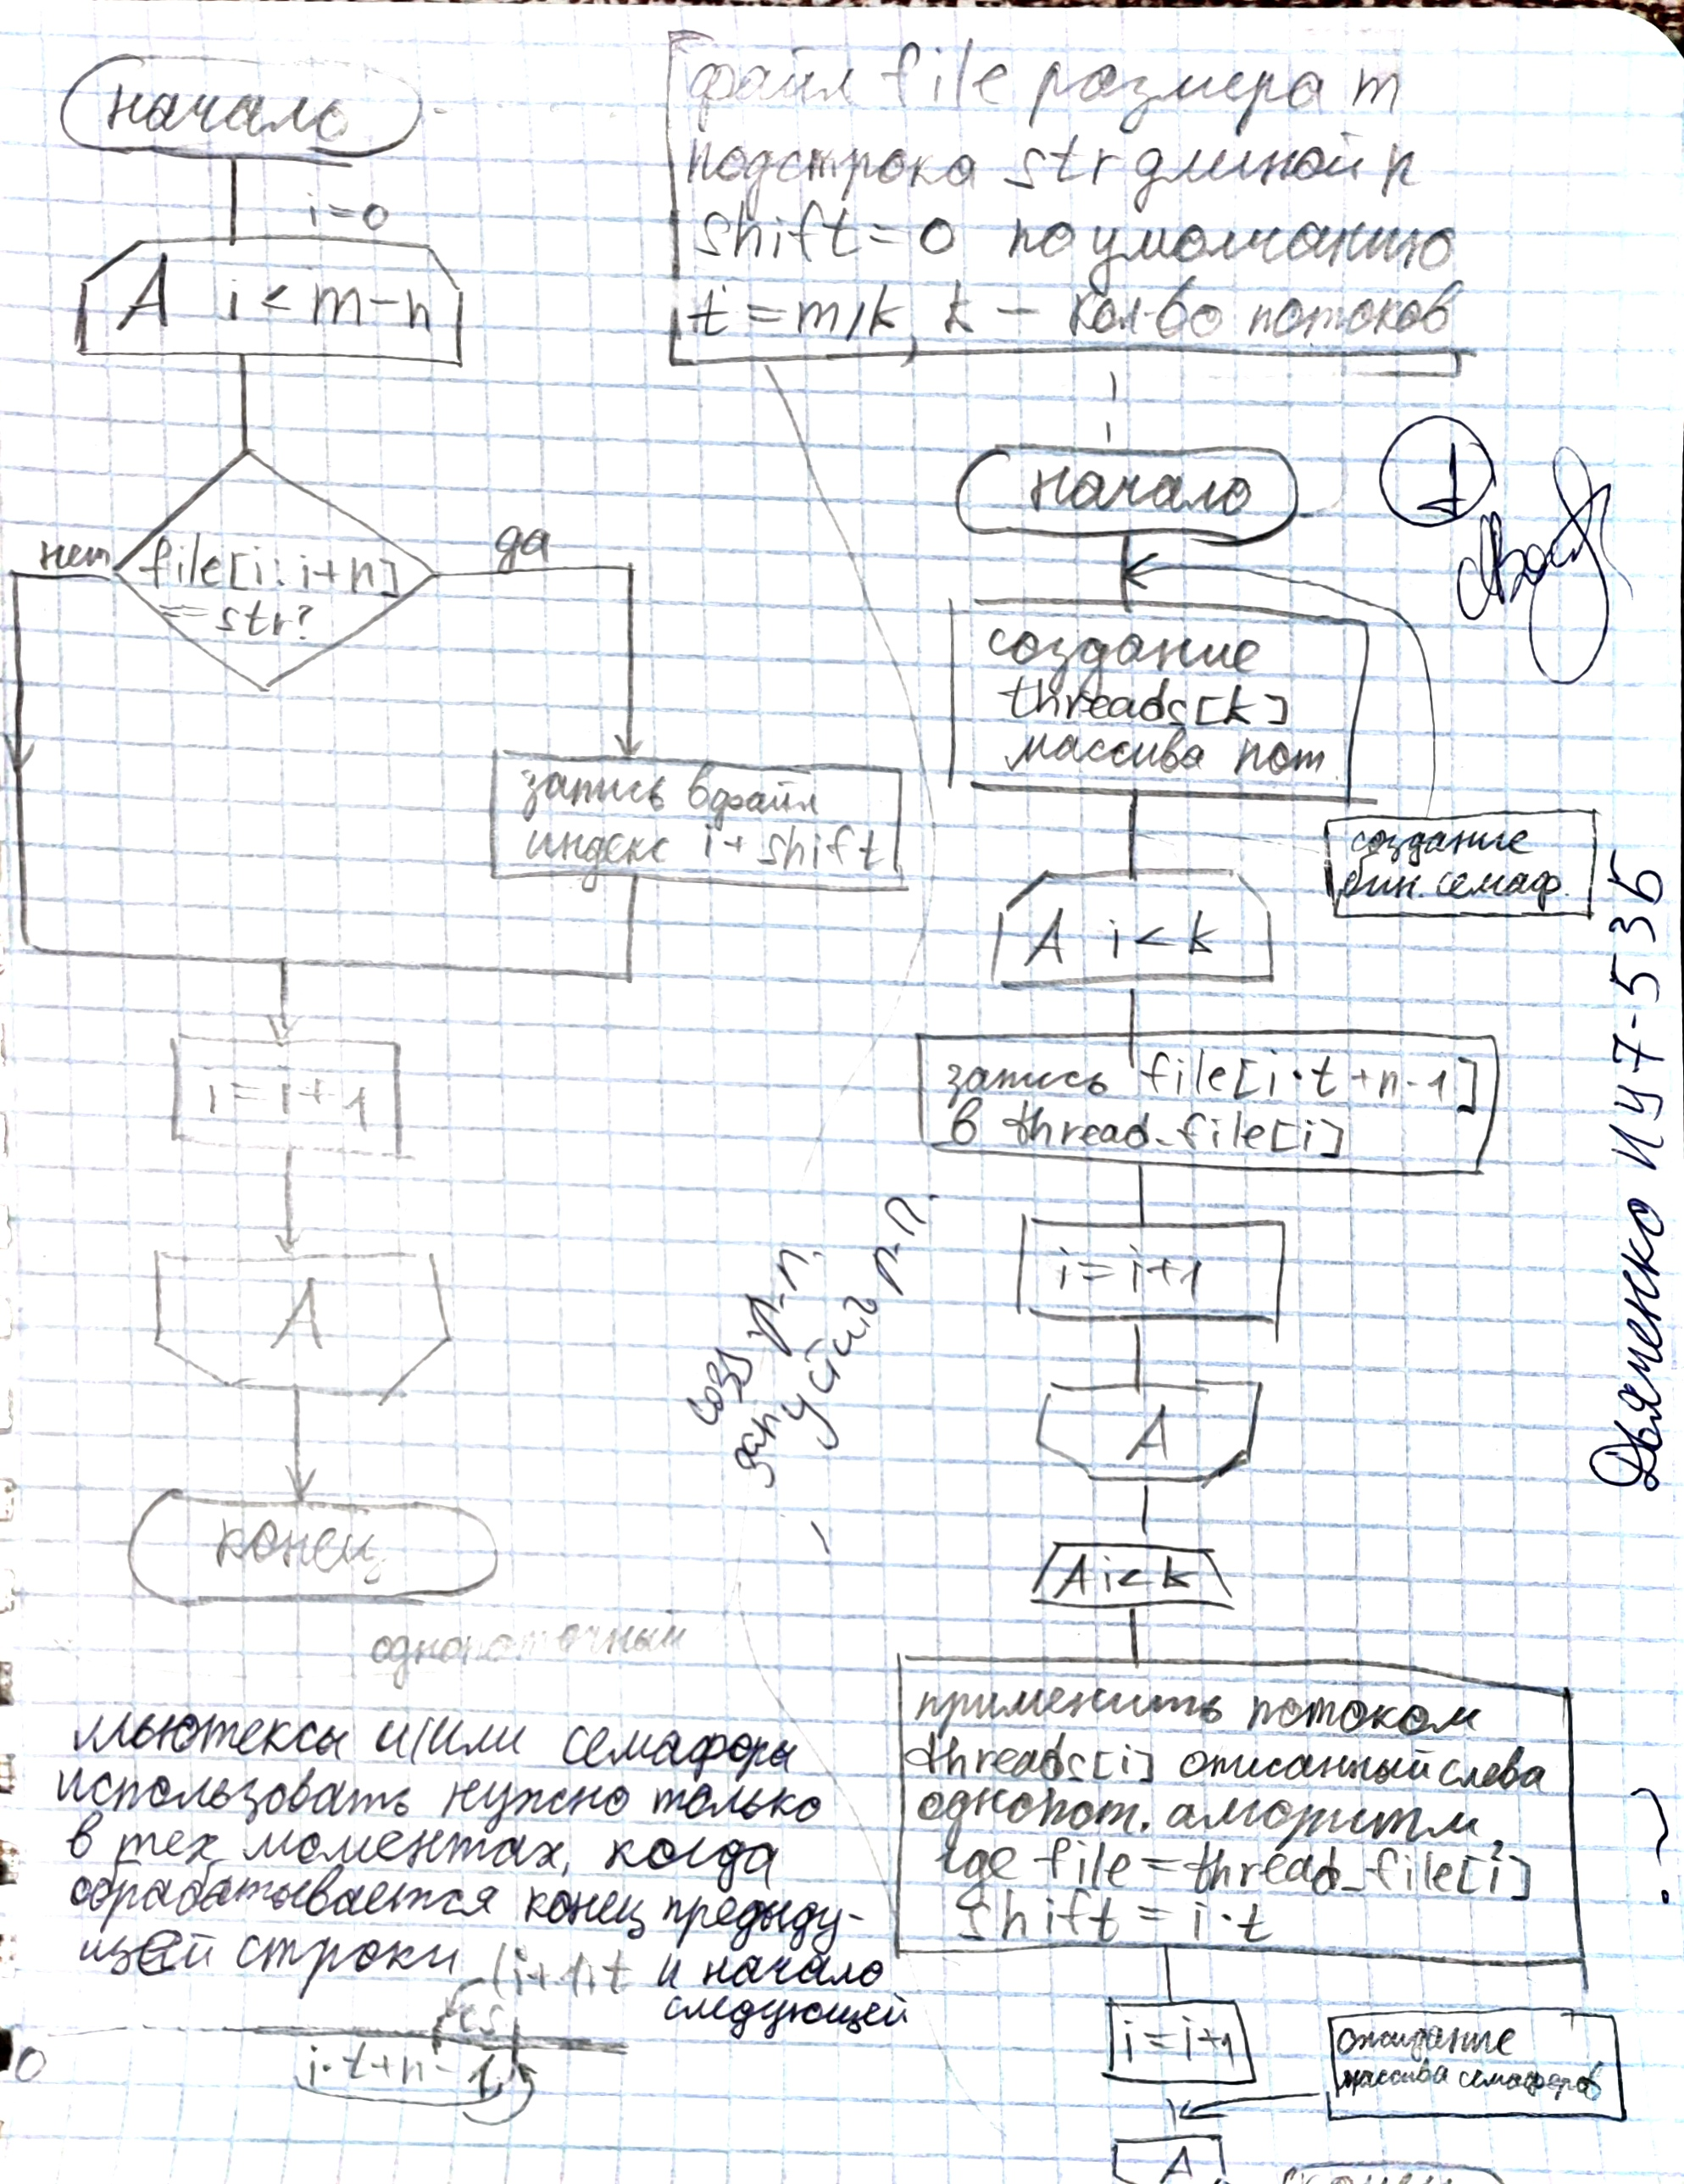
\includegraphics[width=0.7\linewidth]{task}
	\caption{Выполнение задания}
	\label{fig:photo}
\end{figure}

Входными данными являются файл и подстрока для поиска в этом файле.
Результат выводится в результирующий файл с указанием индекса символа, с которого
начинается искомая подстрока (нумерация начинается с 0).

Слева на рисунке расположен алгоритм поиска подстроки в строке.
Справа --- алгоритм главного потока, который инициализирует потоки и контролирует их завершение.

Снизу описан способ контроля доступа потоков к разделяемым ресурсам.
	\section*{ЗАКЛЮЧЕНИЕ}
\addcontentsline{toc}{section}{ЗАКЛЮЧЕНИЕ}

Цель работы достигнута, следующие задачи выполнены:
\begin{itemize}
	\item описана схема последовательного алгоритма поиска подстроки в строке методом полного перебора;
	\item разработано многопоточная версия данного алгоритма;
	\item описана схема алгоритма работы главного потока, который создаёт и запускает вспомогательные потоки;
	\item описана схема алгоритма вспомогательного потока;
	\item обоснована необходимость использования мьютексов и/или семафоров как примитивов синхронизации.
\end{itemize}


	\printbibliography
	
	
\end{document}